\begin{figure}[p]
  \centering
  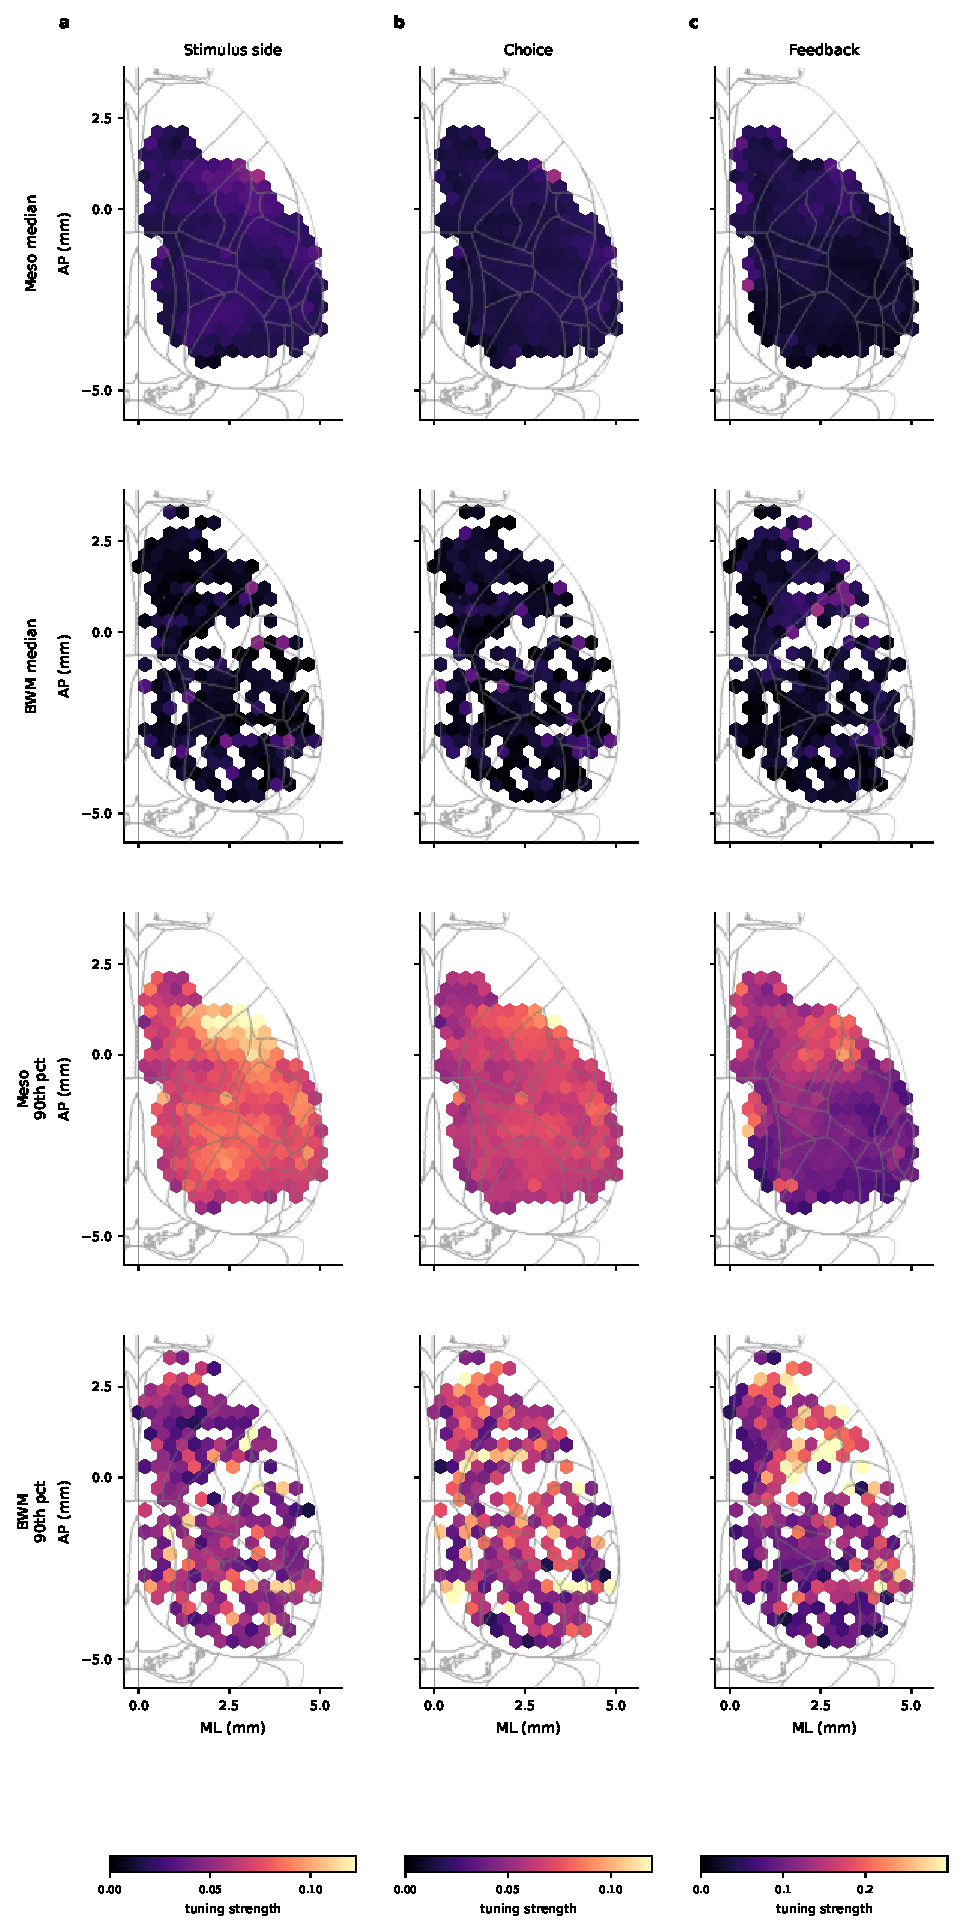
\includegraphics[width=7.00in,height=0.78\textheight,keepaspectratio]{si/si_tuning_strength_panels.pdf}
  \caption{Tuning strength instead of the fraction of significant neurons. For each neuron, the strength is the condition-combined separation of the two conditions (|AUC $-$ 0.5|, pooled over strata, from the same Mann--Whitney statistic as the test) minus its mean over the block-wise shuffles, so 0 is chance and the value does not grow with fewer trials. Rows: median and 90th percentile per bin, mesoscope and BWM; bins with $\geq$10 neurons pooled across sessions; hemispheres folded, 0.4\,mm bins. Colour scales shared within a column. \textbf{a} Tuning strength for stimulus side. \textbf{b} Same for choice. \textbf{c} Same for feedback.}
  \label{fig:si_tuning_strength}
\end{figure}
